\chapter{Section 3:  Creating a Quantified Yolngu Calendar}
The mixed methods, results, and interpretive discussion.

\section{Methods}
-	Briefly describe interview technique to elicit details, how coded in transcripts/notes
-	Touch on literature for seasonal onset detection (eg monsoon).  Stats with time series and missing data are also relevant.
-	Three approaches minimum:  traditional, and others discussed with SCU
-	Describe statistical approaches and meta-method for using them all
-	Outline how to select, normalise, check input data (eg comparison across stations)

\begin{figure}[h]
    \centering
    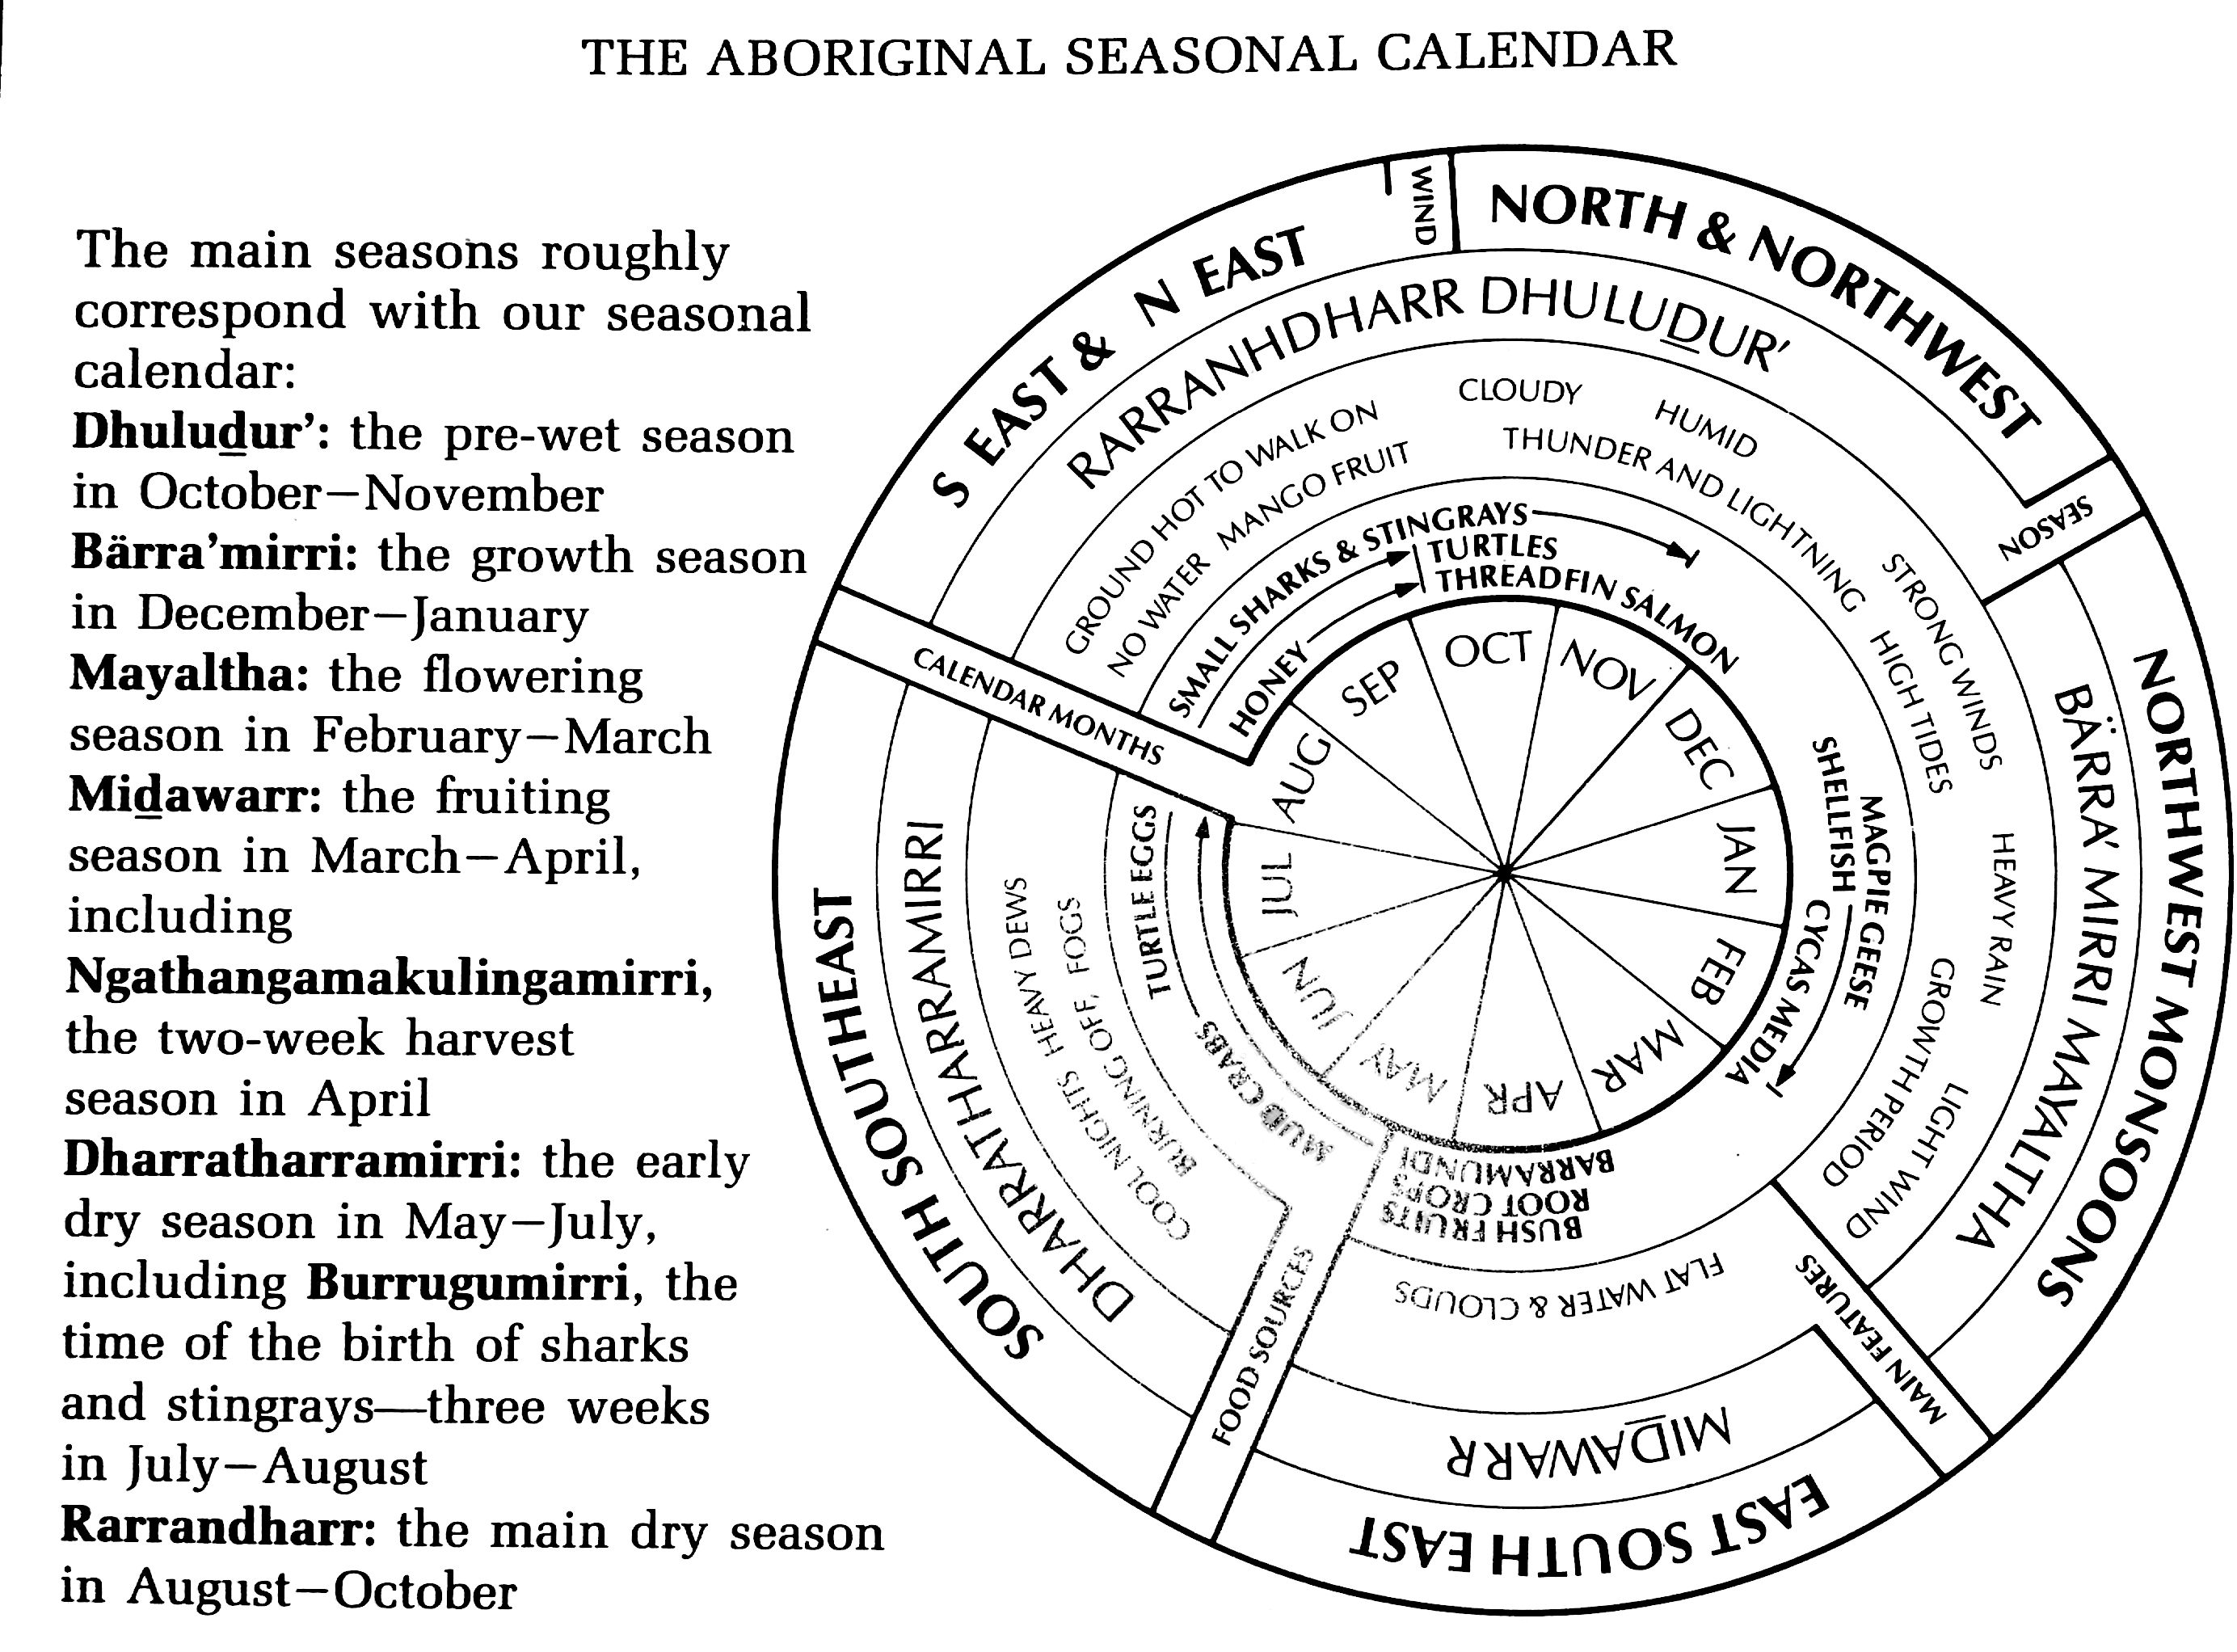
\includegraphics[width=0.8\textwidth]{yolngu-calendar.jpg}
    \caption{Conceptual Yolngu seasonal calendar \citep{davis1989}}
    \label{fig:yolngu-seasons}
\end{figure}

\section{Results and Discussion}
1.	The six seasons are <> (see above).  They are defined by <>.  This calendar has the following interesting properties:  (eg – variable onset, multiple occurrence, at-least-once by climate not construction).
2.	Summary statistics (as charts) for input data, ie weather observations.
3.	For each season:
a.	Determine seasons by each approach, and discuss reliability
4.	<approach> is best, for <reasons>.  Finer distinctions if applicable.
5.	The Quantified calendar is as follows:  <> (with detection functions)

\begin{figure}[h]
    \centering
    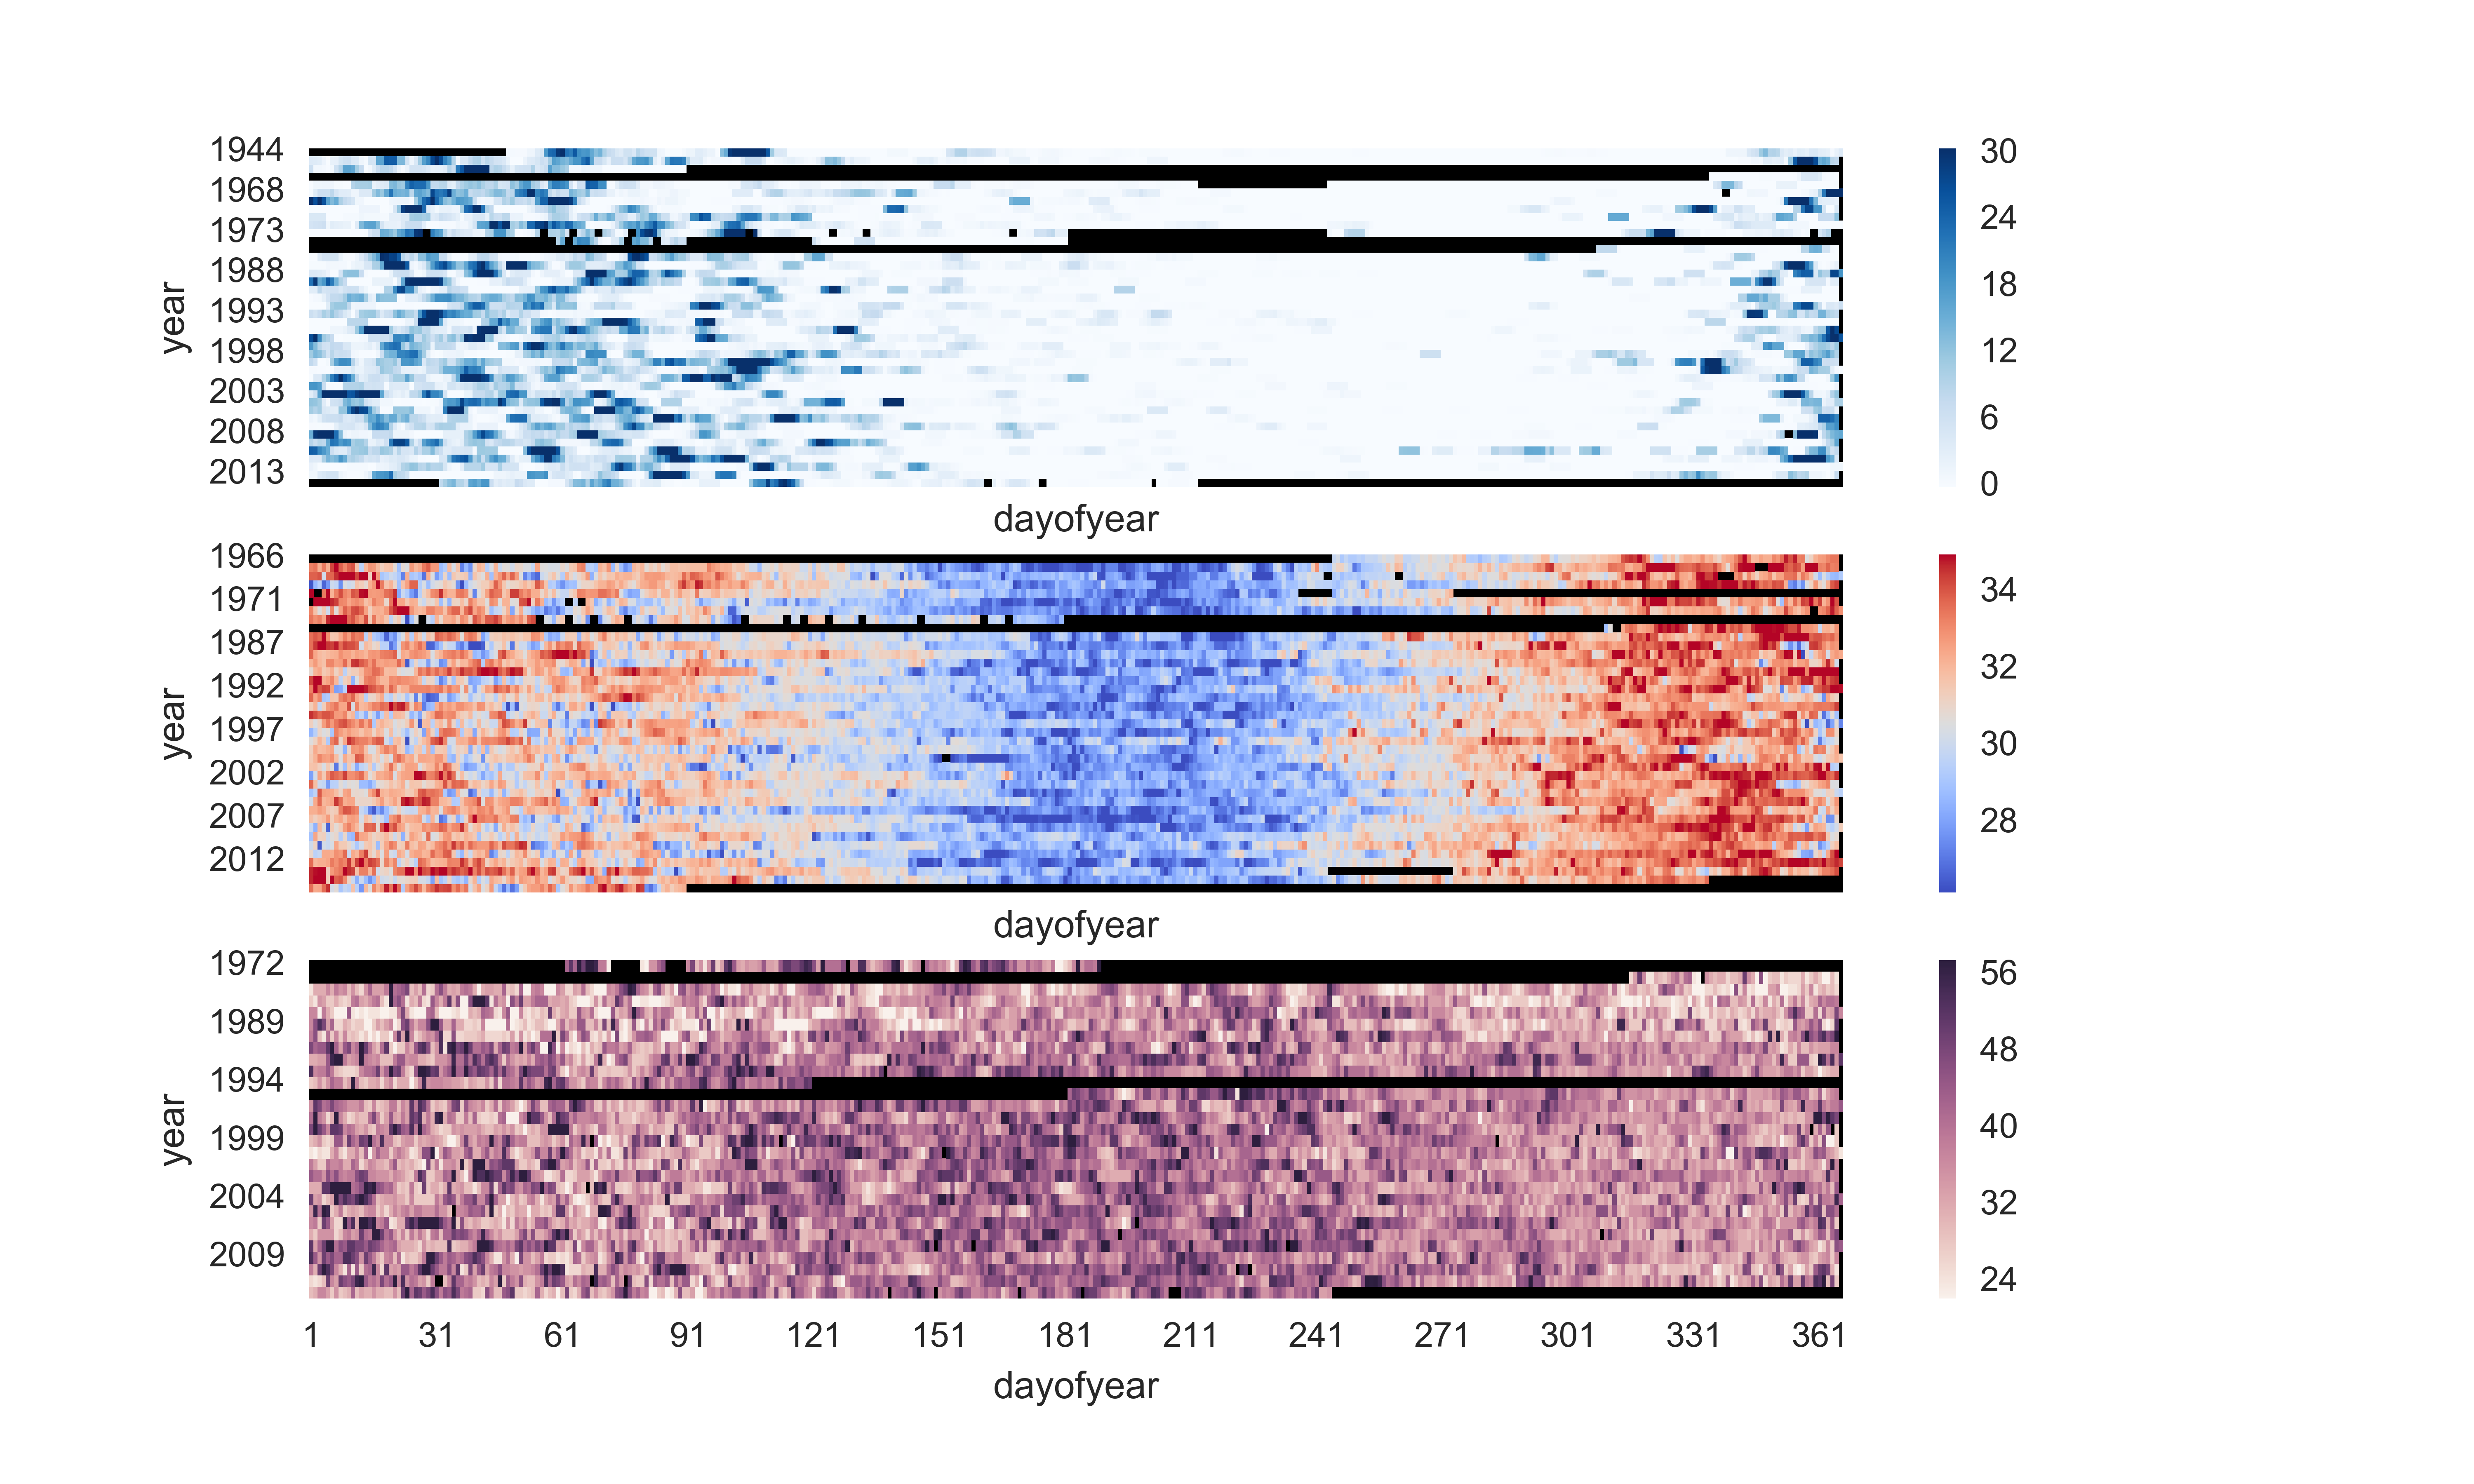
\includegraphics[width=\textwidth]{myfig.png}
    \caption[Rainfall, Temperature, and Wind at Elcho Island]{From top to bottom: Rainfall, Temperature, and Wind at Elcho Island.  Each panel shows one variable, with years on the y axis and day-of-year on the x axis, and observation given by colour intensity.  Note the clear seasonal pattern in rain and temperature.}
    \label{fig:observation-panels}
\end{figure}




